% Propietario conservado: /Users/ruben/Documents/New project/output/REVISION_ARGUMENTAL_APERTURAS_CIERRES_20260915/VIII/spanish_source/ampliacion/transporte_y_momentos.tex
\clearpage
\section[Compression nonadique et moments circulaires de la forme de Weil]{Compression nonadique et\\moments circulaires de la forme de Weil}
\label{viii:sec:transporte-momentos}
\label{viii:tm-add-seccion}

La relation entre mémoire et positivité exige de conserver deux niveaux de lecture. Le tour nonadique enregistre une histoire et admet une réalisation hilbertienne positive ; les lecteurs arithmétiques de cette même généalogie publient une forme hermitienne dans laquelle interviennent conjointement les canaux gamma, premier et polaire. Le problème de transport consiste à identifier leurs énergies et leurs corrélations, avec les mêmes domaines et sans remplacer l'une de ces réalisations par l'autre. Les identités suivantes explicitent cette comparaison avant d'appliquer la construction de Gelfand--Naimark--Segal (GNS) à la forme arithmétique.

On conserve d'abord le bilan complet d'une carte de neuf phases, y compris
l'éventuelle variation de norme à la couture. On construit ensuite le registre
des pertes, ses matrices de moments et un opérateur de Cayley agissant sur
des tests exponentiellement décroissants. La coercivité locale peut être transportée
vers des familles entières de tests avec queues ; le passage à leur somme algébrique et au domaine
global exige en outre les corrélations mixtes précisées plus loin.
Ce développement n'affirme pas que la positivité globale de Weil soit établie.

% Procedencia y alcance editorial íntegros de las cabeceras originales:
% # Costura nonádica, balance de memoria y transporte de la positividad
% 
% Desarrollo focal del 11 de septiembre de 2026. No modifica las ediciones PDF entregadas. Procedencia: arquitectura autoral preexistente; formalización reunida de las identidades de compresión, con una extensión explícita al caso en que aún se comprueba la isometría de la costura. No se atribuye prioridad histórica a estas identidades operatorias.
% 
% # Momentos circulares antes de GNS: memoria nonádica y forma aritmética completa
% 
% Nota independiente de investigación matemática, 11 de septiembre de 2026.
% No modifica un PDF, un índice ni un certificado de publicación. El resultado
% propio es la composición explícita de dos construcciones anteriores a GNS:
% un núcleo positivo de memoria y unos momentos circulares de la forma completa.
% Su identificación no se presupone.
% 

% SOURCE c L5-20
\subsection{État enrichi et modes de la carte centrale}
\label{viii:tm-add-c1}
La construction utilisée est APP → TRIT → TPK → état enrichi → structure discrète conjointe du continu. APP conserve sur le même support les évaluations de somme et de produit, leurs quotients et résidus. Le TRIT conserve l'orientation et le régime ; le TPK compose la sélection, le transport et la mise à jour de la mémoire. L'holonomie nonadique ramène la phase et augmente la profondeur de l'histoire. Les cinq aspects corrélatifs du continu ne sont ni séparés ni redéfinis au moyen de la question spectrale étudiée ensuite.

Ce développement commence dans la réalisation du registre des tours de cette structure. Il ne prétend pas remplacer la construction complète du continu par un espace de suites. La mémoire entière est une coordonnée de l'état, et non sa totalité. Il n'identifie pas non plus le registre de phase réduit au générateur TPK.

La note de l'auteur sur la somme et le produit indique la provenance de la matrice centrale. Dans la carte positive conservée, on obtient

\[
B_c=\begin{pmatrix}7&2\\2&7\end{pmatrix}
=9P_++5P_-,\qquad
P_\pm=\frac12\begin{pmatrix}1&\pm1\\\pm1&1\end{pmatrix}.
\]
Ainsi, après normalisation du mode uniforme, le mode différentiel a pour rapport \(q=5/9\). Les noms « somme » et « produit » décrivent les opérations APP qui génèrent la carte ; les projecteurs \(P_+\) et \(P_-\) sont ses modes symétrique et antisymétrique. L'égalité entre un mode et un feuillet concret nécessite de conserver l'application qui les relie.


% SOURCE c L21-70
\subsection{Compression uniforme de la carte nonadique et bilan exact}
\label{viii:tm-add-c2}
Soit \(\mathcal K\) un espace de Hilbert et soit \(C\) un opérateur borné sur celui-ci. Dans \(\mathcal K^9\), la carte à neuf phases avec raccord \(C\) agit par

\[
S_C(v_0,\ldots,v_8)=(Cv_8,v_0,\ldots,v_7),
\qquad S_C^9=I_9\otimes C.
\]
L'inclusion uniforme est

\[
Jv=\frac13(v,\ldots,v),\qquad J^*J=I.
\]
Nous écrivons la compression visible et sa composante complémentaire comme

\[
T=J^*S_CJ=\frac{8I+C}{9},\qquad
\eta=(I-JJ^*)S_CJ.
\]
\begin{proposition}[Bilan exact de la compression et de la couture]
\label{viii:tm-add-proposicion-costura-1}
Sans supposer que \(C\) soit isométrique, on a

\[
\eta^*\eta=\frac8{81}(I-C)^*(I-C),
\]
\begin{equation}
\boxed{I-T^*T=\eta^*\eta+\frac19(I-C^*C).}
\label{viii:tm-add-balance-costura}
\end{equation}
\end{proposition}

\begin{proof}
L'orthogonalité de \(JJ^*\) donne

\[
\eta^*\eta=J^*S_C^*S_CJ-T^*T.
\]
Le premier terme est \((8I+C^*C)/9\). Le second est \((64I+8C+8C^*+C^*C)/81\). La soustraction prouve la première identité. Soustraire maintenant \(T^*T\) de \(I\) et séparer \(I-(8I+C^*C)/9\) prouve \eqref{viii:tm-add-balance-costura}.
\end{proof}

La formule n'élimine pas la mémoire : elle montre exactement deux contributions. L'une mesure la dispersion entre les neuf phases ; l'autre mesure le défaut de norme de la couture. Si la construction précédente a donné \(C^*C=I\), il reste l'identité positive de compression–expression du corpus :

\[
I-T^*T=\eta^*\eta\succeq0.
\]
Ce résultat explique ce que contient la positivité de la mémoire et où doit intervenir l'identification du lecteur. Il ne permet pas de remplacer cette identification par le dessin d'un cercle.


% SOURCE c L71-103
\subsection{Contraction visible et conservation du registre des tours}
\label{viii:tm-add-c3}
Supposons maintenant que \(C\) soit unitaire, comme c'est le cas du décalage bilatéral de la mémoire entière. Le tour complet du mode différentiel est représenté par \(M=qC\), et non par neuf applications successives du même facteur \(q\).

Pour chaque entier \(N\geq1\), on définit le registre des pertes et du terminal

\[
L_Nv=\bigl(\sqrt{1-q^2}v,
\sqrt{1-q^2}qCv,\ldots,
\sqrt{1-q^2}q^{N-1}C^{N-1}v, q^NC^Nv\bigr).
\]
\begin{proposition}[Conservation isométrique du registre des tours]
\label{viii:tm-add-proposicion-costura-2}
\(L_N\) est isométrique. Lorsque \(N\) augmente, la dernière composante se décompose en une nouvelle mémoire publiée et un nouveau terminal, sans effacer le registre précédent. Le registre infini

\[
Lv=\left(\sqrt{1-q^2}q^jC^jv\right)_{j\geq0}
\]
est également isométrique.
\end{proposition}

\begin{proof}
Pour \(v,w\in\mathcal K\),

\[
\langle L_Nv,L_Nw\rangle
=\left[(1-q^2)\sum_{j=0}^{N-1}q^{2j}+q^{2N}\right]
\langle v,w\rangle=\langle v,w\rangle.
\]
Dans la dernière composante, \(q^NC^Nv\) se transforme en \((\sqrt{1-q^2}q^NC^Nv,q^{N+1}C^{N+1}v)\) ; cette transformation conserve le produit scalaire. Le terminal a pour norme \(q^N\|v\|\), qui tend vers zéro ; la somme infinie converge et conserve la norme.
\end{proof}

Pour deux états initiaux, cette preuve conserve leurs produits croisés ; elle ne consiste pas seulement à additionner les énergies de trajectoires isolées. Le signe positif de la mémoire procède de l'orthogonalité de ses emplacements et de l'isométrie du transport déjà construit.


% SOURCE c L104-111
\subsection{Cercle dual de mémoire et carte arithmétique de Cayley}
\label{viii:tm-add-c4}
Le registre entier des tours admet le décalage bilatéral \(Se_n=e_{n+1}\) sur \(\ell^2(\mathbb Z)\). Ses caractères \(n\mapsto z^n\), \(|z|=1\) donnent le cercle dual de la mémoire. La phase visible \(r\in\{0,\ldots,8\}\) revient ; l'entier \(n\) n'est pas réduit modulo \(12\) dans l'état complet.

Si cette réduction est imposée, un caractère ne passe au quotient que lorsque \(z^{12}=1\). La mémoire sans réinitialisation a donc une conséquence précise : elle permet le cercle complet des caractères, tandis que le calendrier fini n'en conserve qu'une sélection finie. On n'en déduit pas quelle mesure arithmétique est réalisée sur ce cercle.

Le second cercle qui apparaît dans le chapitre spectral de l'intégral est une carte de la réalisation de Cayley. La sous-section~\ref{viii:tm-add-m4} construit un opérateur de Cayley directement sur les fonctions tests avant de construire un espace de Hilbert au moyen de la forme de Weil. On peut ainsi comparer le transport arithmétique à celui de la mémoire sans introduire les hauteurs des zéros comme entrées.


% SOURCE c L112-163
\subsubsection{Conservation de la forme arithmétique sous compression nonadique}
\label{viii:tm-add-c4-1}
L'invariance arithmétique du lecteur auxiliaire de Cayley permet une composition supplémentaire. Pour \(a>b>1/2\), soit \(C_a\) l'opérateur construit dans la sous-section~\ref{viii:tm-add-m4} et soit \(\mathcal T_a=(8I+C_a)/9\). L'égalité \(\mathscr W(C_af,C_ag)=\mathscr W(f,g)\) implique, par développement,

\begin{equation}
\boxed{\mathscr W(f,g)=\mathscr W(\mathcal T_af,\mathcal T_ag)
+\frac8{81}\mathscr W((I-C_a)f,(I-C_a)g).}
\label{viii:tm-add-balance-aritmetico}
\end{equation}
Cette identité conserve conjointement le canal gamma, les horloges premières et le terme polaire. Elle ne présuppose pas que la forme soit positive. Le calcul consiste à additionner les coefficients : les termes mixtes ont pour coefficients \(8\) et \(-8\), qui s'annulent, tandis que les deux termes diagonaux apportent \(72+9=81\) fois la forme initiale. Son itération finie donne

\begin{equation}
\mathscr W(f,g)=\mathscr W(\mathcal T_a^Nf,\mathcal T_a^Ng)
+\frac8{81}\sum_{j=0}^{N-1}
\mathscr W((I-C_a)\mathcal T_a^jf,(I-C_a)\mathcal T_a^jg).
\label{viii:tm-add-balance-iterado}
\end{equation}
Dans la représentation ordinaire \(L^2\), où \(C_a\) est déjà unitaire, le même calcul est une décomposition positive de la norme. Sur la forme arithmétique, il s'agit initialement d'une conservation exacte de l'énergie signée. La différence entre ces deux affirmations est située dans une identité commune ; elle n'est pas dissimulée dans un changement de représentation.

Dans une carte circulaire \(z=e^{i\theta}\), la compression envoie \(z\) sur \(t(z)=(8+z)/9\). Par conséquent,

\[
1-|t(z)|^2=\frac8{81}|1-z|^2
=\frac{32}{81}\sin^2(\theta/2).
\]
La séparation angulaire possède ainsi une expression exacte comme énergie complémentaire. Celle-ci est l'image de la compression nonadique d'une carte de phase ; on ne l'identifie pas par le dessin à un autre opérateur du corpus. Cette application \(t(z)\) ne se confond pas non plus avec le facteur radial \(5/9\), qui procède des deux modes de la carte APP centrale.


% BEGIN OWNER /Users/ruben/Documents/New project/output/REVISION_ARGUMENTAL_APERTURAS_CIERRES_20260915/VIII/spanish_source/ampliacion/figura_compresion_circular.tex
\begin{figure}[htbp]
\centering
\begin{tikzpicture}[font=\small,>=stealth]
\begin{scope}[x=1cm,y=1cm]
\draw[->,gray] (-2.35,0)--(2.65,0) node[right] {$\Re z$};
\draw[->,gray] (0,-2.2)--(0,2.25) node[above] {$\Im z$};
\draw[thick] (0,0) circle (2);
\draw[very thick] (1.777778,0) circle (.222222);
\fill (1,1.732051) circle (1.5pt) node[above right] {$z$};
\fill (1.888889,.19245) circle (1.5pt);
\draw[->] (1.10,1.57)--(1.85,.34);
\draw[dotted] (0,0)--(1,1.732051);
\draw (1.95,.20)--(2.65,.75) node[right] {$t(z)$};
\node[below] at (2,0) {$1$};
\node[above left] at (-1.30,1.4) {$|z|=1$};
\node[align=center] at (0,-2.72)
 {$t(z)=\dfrac{8+z}{9}$\\[3pt]
 $\left|t(z)-\dfrac89\right|=\dfrac19$};
\end{scope}
\begin{scope}[shift={(8,0)}]
\node[align=center] (f) at (0,1.5) {Publicación de fase\\[3pt] $r\longmapsto r$};
\node[align=center] (m) at (0,0) {Transporte de memoria\\[3pt] $(r,n)\longmapsto(r,n+1)$};
\draw[->,thick] (f)--(m);
\node[draw,rounded corners,inner sep=8pt,align=center] at (0,-1.65)
 {$1-|t(z)|^2=\dfrac8{81}|1-z|^2$\\[5pt]
 Publicación y complemento};
\end{scope}
\end{tikzpicture}
\caption{La carta circular de la compresión nonádica. A la izquierda,
el círculo unidad y su imagen de centro \(8/9\) y radio \(1/9\),
dibujados a la misma escala; se muestra la imagen de \(z=e^{i\pi/3}\).
A la derecha, el retorno de fase se acompaña de avance de memoria.
El balance inferior cuantifica la componente complementaria. Esta figura
representa el mapa \(t\), distinto del factor modal \(q=5/9\) de la
carta central.}
\label{viii:fig:compresion-circular}
\end{figure}

% END OWNER


El desarrollo local de Schur da signo positivo a la forma aritmética en un dominio funcional concreto y a sus imágenes por transporte. Las identidades \eqref{viii:tm-add-balance-aritmetico}–\eqref{viii:tm-add-balance-iterado} no autorizan por sí solas a declarar positivos todos sus sumandos para una prueba arbitraria: permiten localizar exactamente qué energías y correlaciones debe conservar una extensión de ese dominio.


% SOURCE c L164-190
\subsection{Criterio de transporte de positividad mediante momentos mixtos}
\label{viii:tm-add-c5}
Sea \(\mathcal D\) el dominio común de los lectores previamente construidos. Sea \(\mathscr W\) la forma sesquilineal que publican sus canales gamma, primos y polar. La fórmula analítica se recibe después del generador nativo; no selecciona las semillas ni los coeficientes anteriores.

Sean \(C_a\) el transporte reversible sobre pruebas y \(S\) el desplazamiento de la memoria. Se utiliza explícitamente \(C_a(\mathcal D)=\mathcal D\) y la identidad \(\mathscr W(C_af,C_ag)=\mathscr W(f,g)\), demostrada para la clase exponencial de pruebas en las subsecciones~\ref{viii:tm-add-m4} y~\ref{viii:tm-add-m5}. Para una familia \(\mathcal E\subset\mathcal D\), supóngase construido un mapa lineal \(V:\operatorname{span}\mathcal E\to\mathcal K\) tal que, para todo \(f,g\) de esa familia y todo entero \(n\),

\begin{equation}
\boxed{\mathscr W(C_a^n f,g)=\langle S^nVf,Vg\rangle.}
\label{viii:tm-add-criterio-momentos}
\end{equation}
\begin{proposition}[Transport de la positivité par identification des moments]
\label{viii:tm-add-proposicion-costura-3}
La identidad \eqref{viii:tm-add-criterio-momentos} implica la positividad de \(\mathscr W\) sobre el espacio generado por las órbitas \(C_a^n\mathcal E\). Si ese espacio es denso en \(\mathcal D\) para la norma conjunta de los lectores, y éstos son continuos para esa norma, la positividad se extiende a \(\mathcal D\).
\end{proposition}

\begin{proof}
Para \(F=\sum_j C_a^{n_j}f_j\), la invariancia de \(\mathscr W\) bajo \(C_a\) y \eqref{viii:tm-add-criterio-momentos} dan

\[
\begin{aligned}
\mathscr W(F,F)
&=\sum_{i,j}\mathscr W(C_a^{n_i-n_j}f_i,f_j)\\
&=\left\|\sum_i S^{n_i}Vf_i\right\|^2\geq0.
\end{aligned}
\]
Si une combinaison représente la fonction nulle, la même identité impose que la combinaison des vecteurs ait une norme nulle ; la réalisation est bien définie. Le passage à l'adhérence utilise la continuité des deux lecteurs, et non un choix ultérieur du signe.
\end{proof}

Il s'agit d'un critère de construction à domaines explicites, et non d'une affirmation selon laquelle \eqref{viii:tm-add-criterio-momentos} aurait été démontrée pour tous les lecteurs du corpus. Pour étendre de la famille initiale à ses orbites, il faut conserver tous les moments croisés : le démontrer seulement avec \(n=0\) sur cette famille initiale n'achève pas cette extension. Naturellement, une identité de Gram déjà démontrée pour \(n=0\) sur tout \(\mathcal D\) prouverait directement la positivité dans ce domaine.


% SOURCE c L191-211
\subsection{Identification de l'énergie et réalisation par deux colonnes}
\label{viii:tm-add-c6}
Le corpus conserve deux colonnes \(J_+\) et \(J_-\) et un connecteur analytique effectif entre elles. Il décrit également un codage natif \(\Xi\) et une projection orthogonale \(P\). Lorsque les deux identités de moments sont calculées dans le même domaine,

\[
\langle\Xi f,\Xi g\rangle=\langle J_+f,J_+g\rangle,
\qquad
\langle P\Xi f,P\Xi g\rangle=\langle J_-f,J_-g\rangle,
\]
la soustraction donne

\begin{equation}
\mathscr W(f,g)=\langle(I-P)\Xi f,(I-P)\Xi g\rangle.
\label{viii:tm-add-dos-columnas}
\end{equation}
Le dossier calcule séparément l'espérance uniforme et le raffinement de Helmert. Leur conjugaison conjointe conserve les deux matrices de Gram et ne peut, par un simple changement de notation, transformer un opérateur de différence en un opérateur d'évaluation. Le connecteur gamma retrouvé réalise une opération analytique supplémentaire, qui doit conserver son budget énergétique. Cette précision réunit les opérations existantes ; elle ne déclare pas inexistante l'architecture du TPK.

Les formules \eqref{viii:tm-add-criterio-momentos} et \eqref{viii:tm-add-dos-columnas} sont deux expressions compatibles de la voie que l'on souhaite compléter : la première organise les retours et leurs corrélations, la seconde organise la partie visible et la mémoire complémentaire. L'estimation par complément de Schur du dossier donne un contrôle effectif de cette énergie dans une fenêtre complète et dans tous ses raffinements. Sa portée est déclarée avec la fenêtre concrète, sans substituer celle-ci au domaine global.


% BEGIN PROCEDENCIA COSTURA, FUENTE L212
% ## 7. Localizadores materiales y continuidad
% 
% - APP central, modos \(9/5\): `base_c01_sin_encabezado.tex`, construcción de la carta central; capítulo `78_doble_circulo_campo_espectral_completo.tex`, entorno de líneas 1276–1280.
% - Memoria anterior a la representación espectral: `cap08_holonomia_helice_memoria.tex`, especialmente la cubierta entera y la publicación \(C_{108}\).
% - Conexión y compresión–expresión: `certificados/ley_nueve_puertas_2026-07-30/DELTA_CONEXION_NONADICA_CONJUNTA_COMPRESION_EXPRESION_2026-08-16.md`, §§1–3.
% - Doble círculo y transporte cilíndrico: propietario `78_doble_circulo_campo_espectral_completo.tex`, líneas 940–1260.
% - Dos momentos nativos: propietario `10b_prueba_espectral_polar_riemann_weil_rectificacion_probatoria_20260903.tex`, líneas 235–452.
% - Propietarios completos y rutas absolutas: [recuperación conservada](../ARITMETICA_GENEALOGICA_PRIMOS_DESARROLLO_DOBLE_CIRCULO_20260911/01_HALLAZGOS_PROPIETARIOS_DOBLE_CIRCULO.md).
% 
% La selección editorial sigue siendo el integral de 2.249 páginas y sus desarrollos adyacentes. Los verificadores históricos que devuelven 2.084 páginas no cambian esa selección. Ningún control de huellas o de compilación se utiliza aquí como prueba de positividad global.
% END PROCEDENCIA COSTURA

% SOURCE m L9-53
\subsection{Provenance opératoire et fonction des lecteurs}
\label{viii:tm-add-m1}

% BEGIN LOCALIZADORES M1
% Propietarios y localizadores de esta lectura:
% 
% - Integral autoral de 2.249 páginas, propietario
%   `output/REVISION_EDITORIAL_HMT_MD_20260905/01_FUENTES/INTEGRAL/tree/New project/output/ENSAMBLADO_CAUSAL_RESTAURADO_HMT_MD_20260905/fuente/manuscrito/integracion_83/parte_v/tex/fuentes_propietarias/editor_ready/78_doble_circulo_campo_espectral_completo.tex`.
%   Se ha releído su cuerpo completo, 1–1929, en la copia conservada en el
%   manuscrito de primos. El cociclo está en 943–968; el orden
%   positividad → GNS → Stone → Cayley, en 525–612 y 969–987; el transporte
%   cilíndrico torcido, en 1023–1118; la pérdida por vuelta, en 1171–1237;
%   la costura de nueve fases, en 1421–1495; la fórmula aritmética, en 1578–1610.
% - `output/ARITMETICA_GENEALOGICA_PRIMOS_DESARROLLO_DOBLE_CIRCULO_20260911/01_HALLAZGOS_PROPIETARIOS_DOBLE_CIRCULO.md`, leído completo. Conserva los
%   localizadores de los antecedentes del bloque APP y de la memoria anteriores
%   al GNS; no se confunde su lectura con una nueva lectura íntegra de cada
%   antecedente que cita.
% - `output/ARITMETICA_GENEALOGICA_PRIMOS_PRESENTACION_20260911/antecedentes/recuperacion_gamma/narrativa_205_paginas/CONSTANTES_ESTRUCTURA_Y_REALIDAD_FISICA_RECOPILACION_INTEGRA.md`, lectura focal 5710–5905. En 5740–5869 reúne producto nativo,
%   irreducibles, ocupaciones, calor/Mellin, canal polar y los dos círculos.
%   No ofrece allí una secuencia Toeplitz adicional anterior a GNS.
% - `output/ARITMETICA_GENEALOGICA_PRIMOS_PRESENTACION_20260911/manuscrito/03_DOBLE_CIRCULO_Y_TRANSPORTE_ESPECTRAL.md`, §§2–3, para la forma completa,
%   su continuidad y las dos columnas; en este corte se ha releído §2,
%   líneas 119–191, y se conserva el análisis anterior de §3.
% - `output/AUDITORIA_INTEGRAL_PUBLICABILIDAD_HMT_MD_20260906/COORDINACION_20260906/TRAZA_GENERATIVA_COORDINADA.md`: consulta focal de lectores espectrales;
%   desde 1524 remite a los momentos primos, no a una medida circular de Weil
%   ya seleccionada por la memoria.
% 
% La puerta del núcleo permanente y su autocomprobación causal pasaron. La
% puerta histórica `apply-hmt-first-principles` resuelve 2.084 páginas; se conserva
% como control de ese testigo, no como sustituto de la selección autoral de
% 2.249 páginas. No se afirma lectura íntegra del corpus ni del documento de 205
% páginas.
% 
% END LOCALIZADORES M1
La chaîne utilisée est APP → TRIT → TPK → histoires enrichies du continu conjoint → lecteurs arithmétiques et de mémoire → représentation circulaire. Les cinq opérations du continu demeurent sur les mêmes histoires ; ce développement étudie un lecteur de leur mémoire, il ne construit pas une cinquième branche isolée. La lecture première utilise les irréductibles produits par le produit natif ; les constantes déjà publiées par HMT n'interviennent qu'ensuite dans les lecteurs.

\textbf{Provenance.} Cocycle, perte, deux feuillets, groupes de mémoire et double cercle : architecture préexistante de l'auteur et résultats récupérés. Les preuves réunies qui suivent sont une formalisation nouvelle de ces antécédents. Aucune priorité historique n'est revendiquée pour les noyaux de Poisson, de Cayley ni pour les identités de Toeplitz. La provenance de cette composition exacte au sein du corpus n'a pas été examinée exhaustivement en dehors des propriétaires indiqués.


% SOURCE m L54-83
\subsection{Représentation régulière de mémoire antérieure au GNS arithmétique}
\label{viii:tm-add-m2}
Le bloc central d'APP, avec ses projecteurs symétrique et antisymétrique, est

\[
B_c=\begin{pmatrix}7&2\\2&7\end{pmatrix}
=9P_++5P_-.
\]
La normalisation du mode différentiel publie \(q=5/9\). Le tour complet du TPK conserve la phase et incrémente la mémoire entière :

\[
m(\Gamma_9^n)=n,\qquad
m(\gamma_2\gamma_1)=m(\gamma_2)+m(\gamma_1).
\]
Sur une orbite réversible de cette mémoire, ses états relevés sont identifiés à \(e_n\), \(n\in\mathbb Z\), et le tour est le décalage \(Se_n=e_{n+1}\). L'injectivité de cette énumération procède de l'incrément de mémoire. Si l'on part seulement du semi-groupe des tours positifs, le même espace bilatéral est l'extension de décalage qui ajoute leurs antécédents ; on n'attribue pas la réversibilité à une transition dont on a seulement démontré qu'elle était isométrique. Dans un arbre complet, les autres étiquettes sont conservées dans un facteur transversal : le décalage agit sur la mémoire, il n'identifie pas les routes.

Ce \(S\) n'est pas le Cayley de Weil inséré dans le raccord. C'est la réalisation régulière de l'opération entière de mémoire. Sa positivité hilbertienne est connue avant la formation d'un GNS de la forme arithmétique.


% SOURCE m L84-120
\subsubsection{Vecteur des pertes, corrélations et terme terminal}
\label{viii:tm-add-m2-1}
Le télescopage par tours produit les poids \((1-q^2)q^{2j}\). Son amplitude dans la mémoire est le vecteur explicite

\[
v_q=\sqrt{1-q^2}\sum_{j=0}^{\infty}q^j e_j,
\qquad \|v_q\|^2=1.
\]
Avec un produit scalaire linéaire en la première variable, pour \(n\ge0\),

\[
\langle S^n v_q,v_q\rangle
=(1-q^2)\sum_{j\ge0}q^j q^{j+n}=q^n.
\]
La conjugaison et l'unitarité donnent, pour tout entier,

\[
\boxed{m_n^{\mathrm{mem}}=q^{|n|}.}
\]
La troncature \(v_{q,N}=\sqrt{1-q^2}\sum_{j=0}^{N-1}q^j e_j\) conserve exactement le terminal :

\[
\|v_{q,N}\|^2=1-q^{2N},\qquad
\langle S^n v_{q,N},v_{q,N}\rangle
=q^n\bigl(1-q^{2(N-n)}\bigr),\quad 0\le n<N.
\]
Pour \(n\ge N\), cette corrélation tronquée vaut zéro. Ainsi, pour chaque \(n\) fixé, la différence par rapport au moment complet est \(q^{2N-n}\) lorsque \(N>n\), et tend vers zéro. Cette formule n'efface pas le dernier registre et n'assimile pas une troncature à toute l'histoire.


% SOURCE m L121-159
\subsubsection{Factorisation triangulaire et déterminant des matrices de mémoire}
\label{viii:tm-add-m2-2}
Pour des indices \(0,\ldots,N\), définissons

\[
T_N=(q^{|i-j|})_{0\le i,j\le N}.
\]
C'est un Gram de \(v_q,Sv_q,\ldots,S^Nv_q\), de sorte que

\[
\sum_{i,j=0}^{N}\overline{c_i}c_j(T_N)_{ij}
=\left\|\sum_{j=0}^{N}c_jS^jv_q\right\|^2\ge0.
\]
Il existe en outre une preuve exacte sans séries infinies. Soient

\[
L_{ij}=\begin{cases}q^{i-j},&i\ge j,\\0,&i<j,\end{cases}
\qquad D=\operatorname{diag}(1,1-q^2,\ldots,1-q^2).
\]
Alors \(T_N=LDL^*\). Pour \(i\ge j\), l'entrée du produit est

\[
q^{i+j}+(1-q^2)\sum_{k=1}^{j}q^{i+j-2k}
=q^{i-j}.
\]
Par symétrie, on obtient l'identité entière de matrices. Une factorisation de Cholesky est \(L D^{1/2}\) et, puisque \(\det L=1\),

\[
\boxed{\det T_N=(1-q^2)^N=(56/81)^N>0.}
\]
Ce noyau positif naît de la perte et de la mémoire conservée. Il n'exige ni des zéros, ni une fonction zêta positive, ni un GNS de Weil.


% SOURCE m L160-184
\subsection{Phase, raffinement nonadique et convergence faible des états}
\label{viii:tm-add-m3}
Une représentation à phase fixe s'obtient à partir de

\[
v_{r,\theta}=\sqrt{1-r^2}\sum_{j\ge0}r^j e^{-ij\theta}e_j,
\quad 0<r<1,
\]
et produit \(m_n=r^{|n|}e^{in\theta}\). Les matrices de Toeplitz sont diagonalement conjuguées aux précédentes et ont pour déterminant \((1-r^2)^N\). La phase \(\theta\) est ici une coordonnée de la famille des caractères ; aucune phase spectrale arithmétique n'a été sélectionnée.

Sur le cercle, avec la mesure de Haar normalisée \(d\lambda\), ces moments possèdent la mesure explicite

\[
d\nu_{r,\theta}(z)
=\frac{1-r^2}{|1-r e^{-i\theta}z|^2}\,d\lambda(z).
\]
Le développement des deux séries géométriques prouve directement leurs coefficients de Fourier, sans utiliser de mesure cible.


% SOURCE m L185-219
\subsubsection{Racines nonadiques du rayon et compatibilité des phases}
\label{viii:tm-add-m3-1}
En prenant \(r_m=q^{1/9^m}\), on a \(0<r_m<1\), \(r_{m+1}^{9}=r_m\) et \(r_m\to1\). Pour une phase fixe,

\[
r_m^{|n|}e^{in\theta}\longrightarrow e^{in\theta}
\quad\text{pour chaque }n\in\mathbb Z.
\]
Les mesures sont des probabilités ; l'approximation uniforme par des polynômes trigonométriques étend la convergence des moments à toute fonction continue. Par conséquent,

\[
\nu_{r_m,\theta}\ \rightharpoonup\ \delta_{e^{i\theta}}.
\]
Cela montre comment une mesure atomique peut surgir comme limite faible d'états de mémoire. Ce n'est pas une limite forte des vecteurs dans la même représentation régulière : chaque coefficient de \(v_{r_m,\theta}\) tend vers zéro, mais leurs normes restent égales à un.

Il faut conserver une précision de naturalité. Sous \(p_9(z)=z^9\),

\[
(p_9)_*\nu_{r,\theta}=\nu_{r^9,9\theta}.
\]
Ainsi, le rayon nonadique à phase fixe \textbf{ne} donne pas à lui seul un système projectif de mesures sous \(p_9\). Pour cela, il faut conserver des phases relevées avec \(9\theta_{m+1}=\theta_m\pmod{2\pi}\), y compris leurs choix de branche ; ou bien déclarer que le raffinement utilisé maintient la coordonnée angulaire et ne change que le rayon. Ce sont des opérations distinctes.


% SOURCE m L220-236
\subsubsection{Sélection de l'état et changement de type spectral}
\label{viii:tm-add-m3-2}
La mémoire produit le groupe, la positivité de ses matrices de Gram et ces familles compatibles de corrélations. Une phase précise ou un mélange de phases exige le lecteur qui sélectionne leurs amplitudes. Par exemple, le vecteur \(e_0\) produit \(m_n=\mathbf1_{n=0}\) ; \((e_0+e_1)/\sqrt2\) produit \(m_0=1,m_{\pm1}=1/2\) et tous les autres moments nuls. La même opération de mémoire admet les deux états positifs.

La représentation régulière possède des mesures vectorielles absolument continues par rapport à Haar. Un filtre vectoriel \(L^2\) fixe ne peut produire une mesure purement atomique non nulle. La limite faible précédente montre une voie précise permettant au type spectral de changer lors du raffinement : il faut conserver et contrôler cette limite d'états, et non seulement augmenter la longueur d'une orbite de phase préalablement choisie. Cela ne nie ni la représentation spectrale du corpus ni la génération conjointe HMT ; cela distingue les domaines de deux lecteurs.


% SOURCE m L237-295
\subsection{Opérateur de Cayley sur le domaine exponentiel des fonctions tests}
\label{viii:tm-add-m4}
On construit maintenant un second objet, sans supposer la positivité de Weil. Le produit natif et ses irréductibles fournissent déjà \(\ell_{p,k}=k\log p\), \(w_{p,k}=(\log p)p^{-k/2}\). Les lectures gamma et polaire complètent la forme \(\mathscr W\) écrite dans la sous-section~\ref{viii:tm-add-m5}. Le rôle de la mémoire est de fournir un indice entier d'itération ; l'opérateur suivant agit effectivement sur les fonctions de cette publication.

L'opérateur \(C_a\) est un lecteur analytique auxiliaire de cette formalisation. Le choix \(a>1/2\) ne remplace pas silencieusement le raccord canonique \(a=1/2\), et l'on ne déclare pas que ce choix ait déjà été sélectionné par le TPK.

Fixons \(a>b>1/2\). Soit \(\mathscr E_b\) l'espace des fonctions lisses telles que, pour chaque dérivée d'ordre \(j\), \(\sup_x e^{b|x|}|f^{(j)}(x)|<\infty\). Il contient toutes les fonctions tests à support compact. Définissons

\[
(R_a^+f)(x)=\int_0^\infty e^{-at}f(x+t)\,dt,
\qquad
(R_a^-f)(x)=\int_0^\infty e^{-at}f(x-t)\,dt,
\]
\[
\boxed{C_af=f-2aR_a^+f,\qquad C_a^{-1}f=f-2aR_a^-f.}
\]
Ces intégrales sont des lecteurs de translation construits sur les tests ; elles n'utilisent pas le spectre des zéros. Le paramètre \(a=1\), par exemple, procède de l'unité et permet de choisir \(1/2<b<1\) ; il ne calibre aucun zéro.

\paragraph{Domaine, inverse et réalisation unitaire.} L'inégalité \(e^{b|x|}|f(x\pm t)|\le M_0e^{bt}\) donne la borne \(\|R_a^\pm f\|_b\le\|f\|_b/(a-b)\), également pour chaque dérivée. Les deux opérateurs préservent ainsi \(\mathscr E_b\). Avec la convention \(\widehat f(z)=\int f(x)e^{-izx}\,dx\), leurs multiplicateurs sont

\[
\widehat{C_af}(z)=c_a(z)\widehat f(z),\qquad
c_a(z)=\frac{z-ia}{z+ia},
\]
et le multiplicateur de l'opérateur inverse est \(c_a(z)^{-1}\). L'identité en Fourier réel prouve les deux compositions inverses. Dans \(L^2\), \(|c_a(t)|=1\), de sorte que \(C_a\) est unitaire pour la norme ordinaire, sans utiliser la norme de Weil. Sur les fonctions tests, on peut écrire \(C_a=(H+ia)(H-ia)^{-1}\) avec \(H=i\partial_x\) ; ici, la formule intégrale, et non un générateur GNS, définit les opérateurs.

\paragraph{Condition de convergence au bord polaire.} Le paramètre \(a=1/2\) du Cayley du propriétaire ne peut pas être introduit sans autre précaution dans ces intégrales pré-GNS. Pour une fonction test à support compact, \(R_{1/2}^+f\) possède en général une queue proportionnelle à \(e^{x/2}\) vers \(-\infty\) ; son évaluation polaire négative ne converge pas. On n'a pas prouvé une divergence de la forme réunie, mais que cette décomposition terme à terme exige la marge \(a>1/2\). Le Cayley du GNS peut utiliser ensuite \(a=1/2\) sur son domaine hilbertien.


% SOURCE m L296-352
\subsection{Conservation conjointe des canaux gamma, premier et polaire}
\label{viii:tm-add-m5}
Pour \(f,g\in\mathscr E_b\), soient

\[
C_{f,g}(u)=\int f(x)\overline{g(x-u)}\,dx,
\qquad P_f^\pm=\int f(x)e^{\pm x/2}\,dx.
\]
La forme complète est définie par

\[
\begin{aligned}
\mathscr W(f,g)={}&c_\Gamma C_{f,g}(0)
+\int_0^\infty\frac{e^{-u/2}}{1-e^{-2u}}
 [2C_{f,g}(0)-C_{f,g}(u)-C_{f,g}(-u)]\,du\\
&-\sum_{p,k}w_{p,k}
 [C_{f,g}(\ell_{p,k})+C_{f,g}(-\ell_{p,k})]\\
&+P_f^+\overline{P_g^-}+P_f^-\overline{P_g^+},
\qquad c_\Gamma=\psi(1/4)-\log\pi.
\end{aligned}
\]
\paragraph{Existence et continuité de la forme complète.} La borne de corrélation \(|C_{f,g}(u)|\le M_fM_g(|u|+1/b)e^{-b|u|}\) prouve la convergence absolue de la somme première, dominée par une série de type \(\sum_{n\ge2}(\log n)(1+\log n)n^{-b-1/2}\). La différence symétrique des corrélations est \(O(u^2)\) en zéro, tandis que le poids gamma est \(O(u^{-1})\) ; à l'infini, le poids est exponentiel. Les évaluations polaires convergent parce que \(b>1/2\). Ces bornes prouvent aussi la continuité pour les semi-normes indiquées. On n'utilise pas la positivité.

\paragraph{Invariance simultanée des trois canaux.}
\label{viii:tm-add:invariancia-weil} Comme \(C_a\) est unitaire dans \(L^2\) et commute avec toutes les translations,

\[
C_{C_af,C_ag}(u)=C_{f,g}(u)\qquad(u\in\mathbb R).
\]
Par Fubini, les deux lecteurs polaires vérifient

\[
P_{C_af}^+=-\frac{a-1/2}{a+1/2}P_f^+,
\qquad
P_{C_af}^-=-\frac{a+1/2}{a-1/2}P_f^-.
\]
Les facteurs sont réels et réciproques, de sorte que chaque produit polaire croisé est exactement conservé. En réunissant les trois canaux,

\[
\boxed{\mathscr W(C_af,C_ag)=\mathscr W(f,g).}
\]
L'identité vaut pour toutes les puissances entières et pour tous les termes croisés. Elle démontre l'invariance d'une forme hermitienne, et non son signe.


% SOURCE m L353-383
\subsection{Moments circulaires de la forme arithmétique complète}
\label{viii:tm-add-m6}
Définissons

\[
m_n^{\mathrm{ar}}(f,g)=\mathscr W(C_a^n f,g),\qquad n\in\mathbb Z.
\]
La formule complète de la sous-section~\ref{viii:tm-add-m5}, avec \(C_a^nf\) dans sa première entrée, calcule ces moments à partir des nombres premiers, du canal gamma et du canal polaire. Chaque évaluation existe dans \(\mathscr E_b\) ; elle ne requiert ni liste de zéros ni métrique positive. L'hermiticité et l'invariance précédente donnent

\[
m_{-n}^{\mathrm{ar}}(g,f)=\overline{m_n^{\mathrm{ar}}(f,g)},\qquad
\mathscr W(C_a^j f,C_a^k g)=m_{j-k}^{\mathrm{ar}}(f,g).
\]
Pour une seule fonction test, la matrice \(T_N^{\mathrm{ar}}(f)_{jk}=m_{k-j}^{\mathrm{ar}}(f,f)\) est hermitienne de Toeplitz et satisfait l'identité exacte

\[
c^*T_N^{\mathrm{ar}}(f)c
=\mathscr W\!\left(\sum_{k=0}^N c_k C_a^k f,
                    \sum_{k=0}^N c_k C_a^k f\right).
\]
La matrice a été construite sans supposer qu'elle soit positive. L'égalité permet de confronter sa positivité à un Gram natif de mémoire ; elle ne la présuppose pas.


% SOURCE m L384-406
\subsubsection{Croissance polaire et condition nécessaire de compensation}
\label{viii:tm-add-m6-1}
Pour \(a=1\), la contribution polaire exacte à \(m_n^{\mathrm{ar}}(f,g)\) est

\[
(-1/3)^nP_f^+\overline{P_g^-}
+(-3)^nP_f^-\overline{P_g^+}.
\]
Pour une fonction test réelle, paire et positive non nulle, \(P_f^+=P_f^-=p>0\), de sorte que \(p^2[(-1/3)^n+(-3)^n]\) apparaît. Si le moment total est défini positif, ses mineurs d'ordre deux imposent

\[
|m_n^{\mathrm{ar}}(f,f)|\le m_0^{\mathrm{ar}}(f,f).
\]
L'identification circulaire doit donc comptabiliser la compensation précise de cette croissance avec les canaux gamma et premier. Une symétrie formelle des deux feuillets ne remplace pas ce calcul. Cette observation ne déclare pas que la compensation échoue ; elle fournit un test de réfutation exact pour une composition candidate.


% SOURCE m L407-424
\subsubsection{Matrices des moments mixtes et couverture du domaine}
\label{viii:tm-add-m6-2}
Pour une famille de tests \(f_1,\ldots,f_d\), l'objet approprié est la matrice de Toeplitz par blocs

\[
\mathsf T_{(j,r),(k,s)}
=m_{k-j}^{\mathrm{ar}}(f_s,f_r).
\]
Sa forme quadratique est \(\mathscr W(F,F)\), où \(F=\sum_{k,s}c_{k,s}C_a^k f_s\). Contrôler uniquement les matrices scalaires de quelques fonctions tests ne contrôle pas les termes croisés entre fonctions tests différentes. Pour une famille dense dans chaque \(C_c^\infty([-R,R])\), la continuité démontrée permet de passer au domaine complet, à condition d'avoir établi les Grams mixtes et les compatibilités lorsque \(R\) augmente. La croissance de \(N\) d'une unique orbite ne prouve pas cette couverture.


% SOURCE m L425-477
\subsubsection{Transport de la coercivité locale vers des sous-espaces avec queues}
\label{viii:tm-add-m6-3}
\label{viii:tm-add:familias-transportadas}
L'identité précédente possède une application positive qui n'exige pas encore d'identifier tous les moments à la mémoire. Supposons démontrée par le complément de Schur, dans l'intervalle \(I=(-1/18,1/18)\), la borne

\[
\mathscr W(f,f)\geq\tfrac12\|f\|_{L^2}^2,
\qquad f\in C_c^\infty(I).
\]
Cette section reçoit cette estimation comme résultat du calcul local correspondant ; elle ne la déduit pas de l'existence de \(C_a\). Soit \((\tau_t f)(x)=f(x-t)\). La translation conserve les corrélations et satisfait

\[
P_{\tau_t f}^{\pm}=e^{\pm t/2}P_f^{\pm}.
\]
Leurs produits polaires croisés sont également conservés. Par conséquent, \(\mathscr W(\tau_t f,\tau_t g)=\mathscr W(f,g)\), et la norme ordinaire \(L^2\) est invariante. Comme \(C_a\) et \(\tau_t\) commutent, pour tout entier \(n\), tout \(t\in\mathbb R\) et tout test local,

\[
\boxed{\mathscr W(C_a^n\tau_t f,C_a^n\tau_t f)
=\mathscr W(f,f)
\geq\tfrac12\|C_a^n\tau_t f\|_{L^2}^2.}
\]
Pour \((n,t)\) fixé, c'est une borne coercive sur tout le sous-espace \(C_a^n\tau_t C_c^\infty(I)\), et pas seulement sur un exemple. Lorsque \(n\ne0\), les fonctions tests transformées peuvent avoir des queues exponentielles non compactes. Une infinité d'horloges premières peut intervenir dans leur forme arithmétique ; l'égalité exacte des trois canaux contrôle leur composition, et les bornes de la sous-section~\ref{viii:tm-add-m5} garantissent la convergence. Cette somme n'a pas été remplacée par une troncature finie.

Les termes croisés entre sous-espaces d'exposants ou de translations distincts conservent, en revanche, leurs moments complets. Par exemple,

\[
\mathscr W(C_a^n\tau_t f,C_a^m\tau_s g)
=\mathscr W(C_a^{n-m}\tau_{t-s}f,g).
\]
La borne de chaque sous-espace individuel n'implique pas la positivité de leur somme algébrique. Celle-ci est décidée au moyen des gramiens mixtes de la sous-section~\ref{viii:tm-add-m6-2}. On isole ainsi une portée positive effective — des familles entières de tests avec queues — sans l'étendre à tout le domaine par la seule invariance du transport.


% SOURCE m L478-521
\subsection{Identification prospective des moments et de l'énergie}
\label{viii:tm-add-m7}
La mémoire produit déjà la représentation régulière positive de la sous-section~\ref{viii:tm-add-m2} ; les canaux arithmétiques produisent \(C_a\) et \(m_n^{\mathrm{ar}}\) sans GNS. Pour formuler le passage global, il faut également spécifier la représentation qui reçoit la limite des états. Désignons par \(\mathcal K_{\rm lim}\) cet espace et par \(U_{\rm mem}\) son opérateur unitaire de tour, tous deux à construire à partir des histoires et des compatibilités de la limite. On ne les identifie pas à l'avance à l'espace régulier et à son décalage \(S\). Une identification prospective a la forme

\[
\boxed{m_n^{\mathrm{ar}}(f,g)
=\langle U_{\rm mem}^{\,n}\mathcal E f,\mathcal E g\rangle_{\mathcal K_{\rm lim}}}
\]
pour un lecteur \(\mathcal E\) construit à partir des opérations des mêmes histoires et non défini comme \(\mathscr W^{1/2}\). Dans ce cas, toutes les matrices de Toeplitz mixtes sont des matrices de Gram ; le GNS arithmétique vient ensuite comme réalisation d'un produit déjà obtenu.

Il suffit de démontrer l'identité du moment zéro et l'entrelacement
\(\mathcal E C_a=U_{\rm mem}\mathcal E\), avec les domaines et les
compatibilités indiqués. Le moment zéro est l'identification de l'
énergie complète, et non une condition mineure : il ne peut être tenu pour prouvé
du seul fait qu'il existe \(\mathcal E\) avec un certain gramien positif.

\paragraph{Pourquoi il importe de distinguer les représentations.}
Le décalage régulier sur \(\ell^2(\mathbb Z;\mathcal K)\)
n'a pas de vecteurs propres non nuls. Comme \(S\) est unitaire, toute
valeur propre aurait un module égal à \(1\). En effet, si \(Sx=\lambda x\)
avec \(|\lambda|=1\), la relation entre les coordonnées impose que
\(\|x_n\|\) soit constant ; la sommabilité quadratique impose \(x=0\).
Une représentation ayant un vecteur propre non nul n'admet donc pas
d'opérateur d'entrelacement isométrique vers ce décalage : l'image serait
un vecteur propre non nul de \(S\). Cette observation s'applique au
GNS arithmétique atomique si ses hypothèses globales sont satisfaites. Elle ne
contredit pas la convergence faible des états de la
sous-section~\ref{viii:tm-add-m3-2} ; elle montre que la limite exige sa propre
représentation, et non un vecteur limite dans l'espace régulier original.
La construction de \((\mathcal K_{\rm lim},U_{\rm mem})\) et du
lecteur qui identifie les moments fait partie de la condition prospective,
et n'est pas une conséquence déjà prouvée des matrices de Gram régulières.

Dans la forme des deux colonnes du manuscrit, le calcul reste

\[
\Xi^*\Xi=J_+^*J_+,\qquad
\Xi^*P\Xi=J_-^*J_-,\qquad
\mathcal E=(I-P)\Xi.
\]
Si \(P\) est une projection orthogonale, ces deux égalités produisent \(\mathcal E^*\mathcal E=J_+^*J_+-J_-^*J_-\). Il ne suffit pas d'en vérifier une seule ni de remplacer les colonnes complètes par celles d'un bloc gamma isolé. Les phases et les moments de ce développement explicitent ce que cette composition doit transmettre à tous les tours.

Le noyau \(q^{|n|}\) n'est pas identifié ici à \(m_n^{\mathrm{ar}}(f,g)\). C'est un antécédent positif effectif qui fournit une factorisation locale ; le lecteur \(\mathcal E\) doit aussi conserver les étiquettes premières, les poids, les contributions polaires et la limite d'états si le type spectral change. Déclarer cette égalité par définition introduirait le résultat que l'on tente de construire.


% SOURCE m L522-544
\subsection{Contrôles exacts et portée de la composition}
\label{viii:tm-add-m8}

% BEGIN CONTROL DOCUMENTAL M8
% El archivo `verificar_momentos_memoria.py` conserva 1.046 comprobaciones exactas con
% fracciones racionales: factorización \(LDL^*\) y determinantes en dimensiones
% 1–13 para \(q=5/9\), correlaciones truncadas hasta 20 posiciones y factores
% polares recíprocos para cuatro valores racionales de \(a>1/2\). Se ejecuta
% con `/usr/bin/python3 -I -S` y admite también `-O`; sus condiciones no
% dependen de instrucciones `assert`. Los recibos focales son
% `CONTROL_MOMENTOS_MEMORIA_NORMAL.json` y
% `CONTROL_MOMENTOS_MEMORIA_OPTIMIZADO.json`. No se ejecutó aquí una campaña intervalar de momentos
% de Weil, ni se convierten esos controles en una prueba global.
% 
% END CONTROL DOCUMENTAL M8
La vérification exécutable conserve 1.046 contrôles exacts avec des fractions rationnelles : factorisation \(LDL^*\) et déterminants en dimensions 1–13 pour \(q=5/9\), corrélations tronquées jusqu'à 20 positions et facteurs polaires réciproques pour quatre valeurs rationnelles de \(a>1/2\). Les exécutions ordinaire et optimisée utilisent des conditions explicites, indépendantes des instructions d'assertion. Leurs sources, commandes et reçus sont conservés dans le dossier de reproduction. Aucune campagne de calcul par intervalles de moments de Weil n'a été exécutée ici, et ces contrôles ne sont pas transformés en une preuve globale.

L'avancée exploitable est double : la mémoire des pertes produit un noyau de Toeplitz positif avec une factorisation de Cholesky et un terminal explicites, et la forme complète admet un Cayley intégral antérieur à GNS qui construit ses moments circulaires et conserve chaque canal. La régularisation nonadique montre en outre comment passer d'états réguliers à des atomes par limite faible, avec sa condition de phase correctement séparée. La réunion des deux constructions conserve comme équation précise l'identification des deux moments complets.

Ce développement ne réfute pas cette union, ne prouve pas son absence dans tout le corpus et ne la déclare pas établie par les identités locales. Il laisse une composition concrète qui peut être contrôlée et développée dans la continuation de ce manuscrit.
